\section{Materials and Methods}
%#######################Ayoub#########################################
\subsection{Hardware}
\subsubsection{Arduino}%a modifier

The Arduino Uno served as a programmed interface between the computer-based control system and the mechanical components of our 3dof Stewart platform, which was at the center of our experimental setup. An Arduino Uno, a board built on the ATmega328P microprocessor, was employed in this study. It includes a 16 MHz quartz crystal, 6 analog inputs, 14 digital input/output pins (of which 6 can be used as PWM outputs), a USB port, a power jack, an In-Circuit Serial Programming (ICSP) header, and a reset button.\cite{atmel_atmega328p_nodate}\newline

The Arduino's ability to translate MATLAB Simulink signals into servo-actionable commands is what makes the experimental setup successful. The Uno was configured to execute these instructions on the 3dof Stewart platform in real-time using the Arduino Integrated Development Environment (IDE). This allowed the PID controller to manage the ball's position.\newline

The maximum current output of the Arduino Uno is one of its drawbacks because it cannot power numerous servos. The Uno's digital or analog pins have a cap on the amount of current they can deliver at roughly 20 mA per pin, with a total output of 200 mA across all pins\cite{atmel_atmega328p_nodate}. This is insufficient for the current-hungry servos utilized in this configuration.


\subsubsection{External Power Supply}

The servos were powered by an external power source in order to get around this restriction. This configuration prevented the Arduino, which would have most certainly led to system failure due to the Uno's power limitations, from supplying the servos with the necessary current.\newline 

To guarantee constant voltage levels and avoid any ground loop issues, the external power supply and the Arduino shared a common ground. This allowed the Arduino to control the servos without also having to supply power for them, ensuring that the Arduino Uno's capabilities were fully utilized within its operational parameters.


\subsubsection{Servos}%a modifier

Servo motors, a class of electric motor devices sometimes referred to as "servos," are used in robotics and other sectors due to their accuracy and control skills. A motor, a control circuit, a potentiometer (for position feedback), and gears are the components of a servo. They may be controlled by providing them a particular electrical pulse signal, and they are made to rotate and retain the output shaft in a given position. They are perfect for applications needing precision positioning since they can hold their position even when outside forces try to shift them.\newline

We used Tower Pro MG995R servo motors for this build. These are metal-geared, high-torque servos that provide greater stability and longevity than their plastic-geared equivalents. They are a great option for demanding applications like ours because of their voltage range of 4.8 - 7.2V and their stall torque of roughly 10 kg-cm (at 6V)\cite{tower_pro_mg995_nodate}.\newline

RC servo pulses with a range of roughly 500 to 2500 microseconds and a refresh rate of about 50 Hz are accepted by the Tower Pro MG995R. The servo can rotate its output shaft to a precise angle within a range of 180 degrees in response to these input pulses.\newline

The Arduino in our setup converted the control directives from the MATLAB Simulink model into the pulse-width modulation (PWM) signals that the servo motors could interpret. The Stewart platform's position was modified by the servos in response to these signals, allowing for fine control of the ball's placement on the platform.\newline

The Tower Pro MG995R servos' sturdy design and good torque performance were crucial in preserving accurate and stable control of the 3dof Stewart platform, highlighting their efficiency in high-precision control systems.

%######################Vincent########################################
\subsubsection{Serial communication}
Serial communication is a form of data transfer where information is transmitted sequentially, one bit at a time, over a single communication channel. It is a fundamental method employed in digital communication systems for the exchange of data between two devices. Serial communication offers several advantages, including simplicity, reliability, and compatibility with a wide range of devices. It is extensively utilized in various applications, such as computer peripherals, embedded systems, and long-distance communication between devices.
\newline
Serial communication was employed in our setup to ensure the reliable and real-time transfer of data between the computer and the Arduino. We used the Arduino's onboard hardware serial ports to communicate with the computer.
Serial communication must be configured on the transmitter(MATLAB Simulink) and on the receiver(Arduino).\newline
\paragraph{MATLAB Simulink side.}
Serial communication requires perfect synchronization between the transmitter and the receiver. The processing time in our algorithm being variable, the use of a Zero-Order Hold (ZOH)\footnote{a Zero-Order Hold (ZOH) approximates a continuous-time signal by maintaining a constant value during each sampling period. } is necessary to guarantee a perfect synchronization. The Simulink program concatenates the desired angle for each of the servos and transmits them at fixed intervals to the Arduino.

\paragraph{Arduino Uno side.}
The Arduino board is configured to read at fixed intervals its serial reception buffer. The reading frequency is the same as the transmission frequency configured in the ZOH. The received angles are decomposed and are finally transmitted to their respective servo.



\subsection{Ball detection}
\subsubsection{Image acquisition}
The camera used is a "Microsoft LifeCam HD-3000", presented in Figure \ref{Microsoft LifeCam HD-3000 Webcam}. It is a generic webcam supporting a resolution of up to 1280x720 pixels\cite{noauthor_microsoft_nodate}. Even though faster technologies exist such as touchscreens\cite{adak2015touchscreen}, we decided
to keep the camera since it is a cheaper alternative and has frames per second (FPS) and latency
properties that are enough for a simple ball detection system.\newline
\begin{center}
    \begin{figure}[ht!]
        \centering
        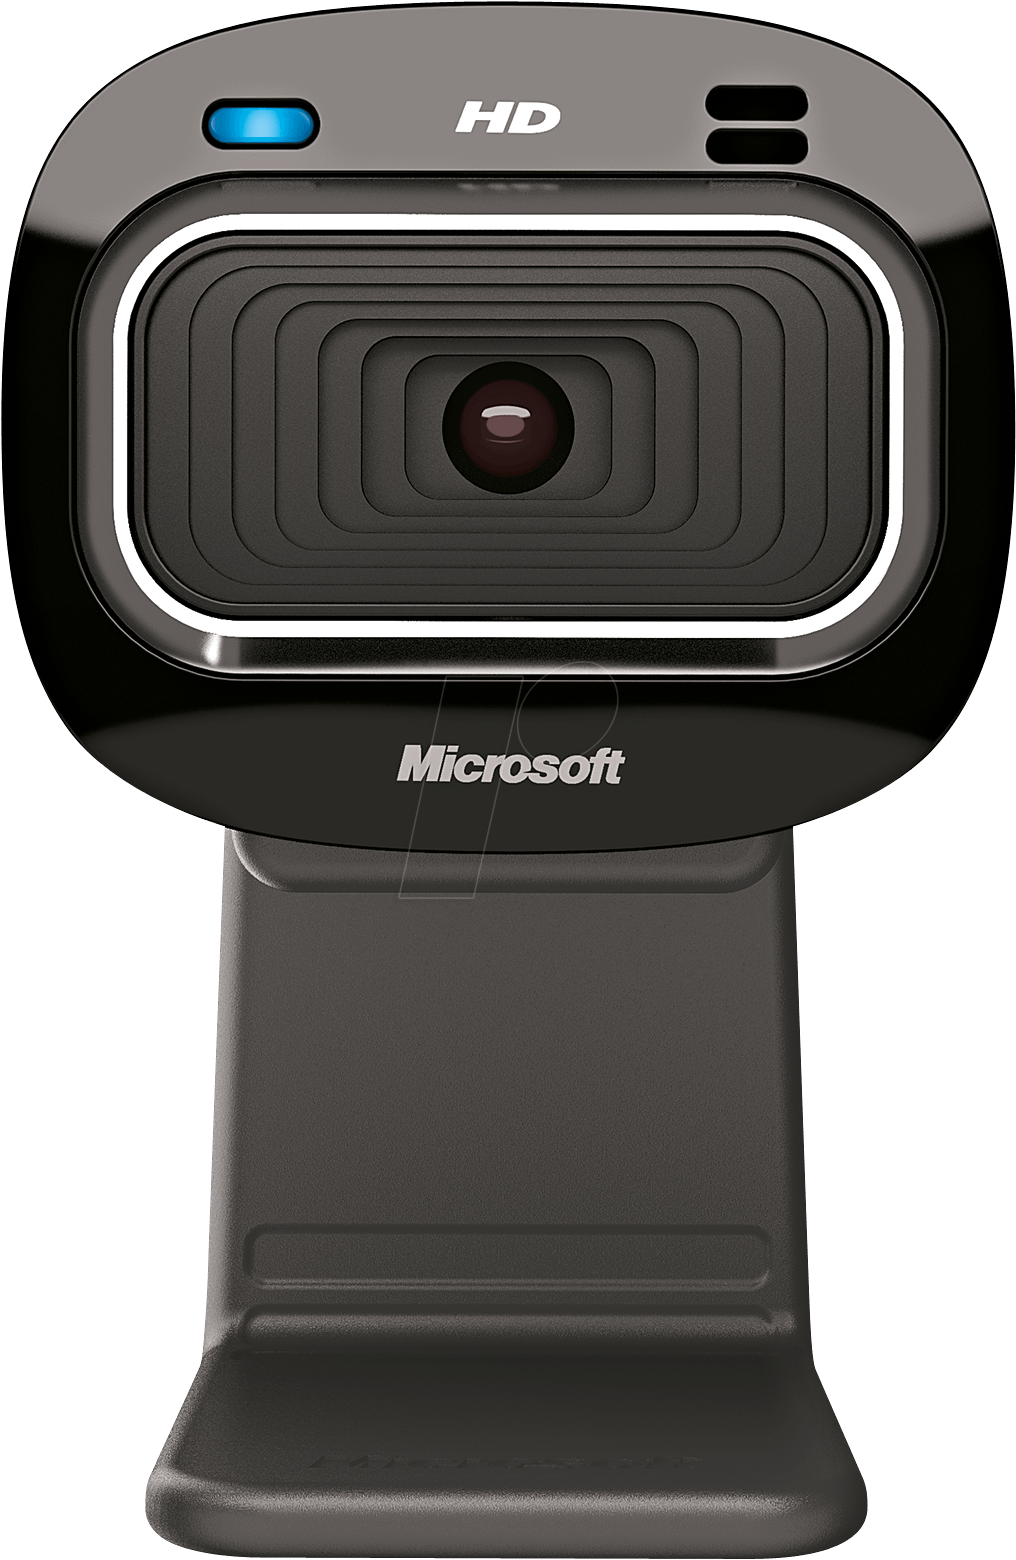
\includegraphics[width=3cm, keepaspectratio]{imports/MS_Lifecam.png}
        \caption{Microsoft LifeCam HD-3000 Webcam \cite{noauthor_microsoft_nodate}}
        \label{Microsoft LifeCam HD-3000 Webcam}
    \end{figure}
\end{center}
    \newpage
  \subsubsection{Description of our image recognition system}
  As our model will be used for practical work, we decided to use exclusively MATLAB Simulink for the whole project. Therefore we have to use it also for the ball detection.\newline
  The camera provides images of the ball on the platform to the MATLAB algorithm and the images are processed using the "Blob Analysis" function\cite{noauthor_statistics_nodate}. In order to keep a simple algorithm and to increase the processing speed, no AI was involved.\newline
  For this reason, we had to pick an orange ball whose color is very different from the white plate. This allowed the algorithm to detect the outline of the ball, and from this outline, to compute the x and y coordinates of the center of the ball.\newline
  

  \subsubsection{The Blob Analysis function}
In MATLAB, the blob analysis function is used to identify and analyze connected regions or "blobs" in an image. Blobs typically represent objects or regions of interest that share similar characteristics, such as color, intensity, or texture.
\newline
The blob analysis function in MATLAB offers several operations to extract useful information from blobs, such as their centroid, area, perimeter, bounding box, and more.
\newline
The following parameters must be chosen to make the algorithm work properly : 
\begin{enumerate}
  \item Allowable color range: In order to recognize only the orange ball, an appropriate color interval must be used. This range must be wide enough to take into account the different brightness conditions. We have chosen an interval from hsv(5,40,50) to hsv(15,100,100), shown in Figure \ref{Allowable color range : from hsv(5,40,50) to hsv(15,100,100)}.
  \begin{center}
    \begin{figure}[ht!]
        \centering
        
\includegraphics[width=10cm, keepaspectratio]{imports/hsv_grad.png}
        \caption{Allowable color range : from hsv(5,40,50) to hsv(15,100,100)}
        \label{Allowable color range : from hsv(5,40,50) to hsv(15,100,100)}
    \end{figure}
\end{center}
  \item Image preprocessing: A x5 numeric zoom is applied in order to only analyze the platform
  \item Bloc Detection: The allowable area range for the object is set [100, 10000] square pixels. The defined interval prevents the system from confusing the ball with very small orange objects (wire, digital noise)
  \item Post-processing: Of all the orange objects that can be identified, only the largest is considered. The function then returns the center of this object.
\end{enumerate}
\subsubsection{User interface}
In order to allow an easy debugging to the user, an interface allowing to visualize in live the images taken by the camera as well as the position of the ball has been added.\newline
A first function named concatenate is in charge of transforming the position (x,y) and the surface of the ball into a shape\newline
The "Draw circle" block allows to overlay the original image with the shape.\newline
The whole set is then displayed to the user thanks to the "To video display" block.\newline
The Simulink blocks used are shown in Figure \ref{Simulink diagram of the interface}.
  \begin{center}
    \begin{figure}[ht!]
        \centering
        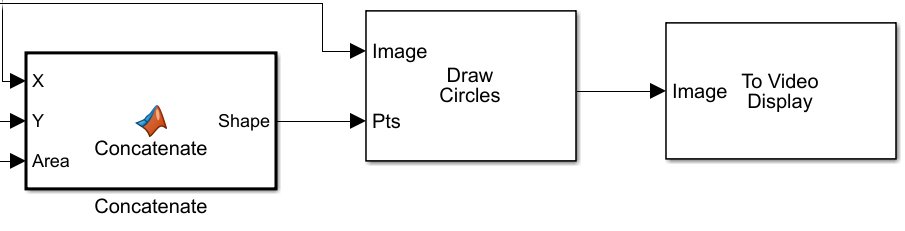
\includegraphics[width=10cm, keepaspectratio]{imports/IHM_simulink.png}
        \caption{Simulink diagram of the interface}
        \label{Simulink diagram of the interface}
    \end{figure}
\end{center}
%######################Eddy and Johan###########################################
\subsection{System modeling}

    \subsubsection{Mathematics modeling}\label{System modeling}

    \paragraph{Illustrative graph}
\begin{center}
      \begin{figure}[h]
    \centering
    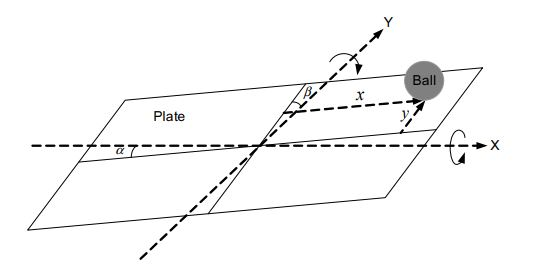
\includegraphics[width=10cm]{imports/Captura.jpg}
    \caption{Free body diagram}
        \label{Free body diagram figure}
    \end{figure}
\end{center}

    \paragraph{Mathematical modeling}
    In this case, we use Newton's second law to the free body diagram presented in Figure \ref{Free body diagram figure}, which states that the sum of forces is equal to mass times acceleration. Applying it to angular acceleration, we obtain the following two differential equations that provide the modeling of the system
    \begin{equation}
    (m+\frac{I}{r^2})\ddot{x}-m(x\dot{\alpha}^2+y\dot{\alpha}\dot{\beta})+mg\sin(\alpha)=0
    \end{equation}
    \begin{equation}
    (m+\frac{I}{r^2})\ddot{y}-m(y\dot{\beta}^2+x\dot{\alpha}\dot{\beta})+mg\sin(\beta)=0
    \end{equation}
    \paragraph{Linearization}
    In general, the dynamics of the ball and plate system can be linearized under the following assumptions: 
    \begin{itemize}
\item The ball is considered as a point object with concentrated mass.
\item The plate is considered rigid and its deformation is negligible.
\item Contact forces between the ball and plate are modeled as normal and tangential forces.
\item Angular accelerations of the ball and plate are small.
\item The angle of rotation of the plate is small so that we can
suppose $\sin{\alpha} \approx \alpha $ and $\sin{\beta} \approx \beta $
\item The centrifugal force on the ball can be ignored as it is very
small compared to gravity.
\end{itemize}
    From these assumptions, the linearized model can be expressed
as following:
\begin{equation}
\ddot{x}+\frac{5}{7}g\alpha=0
\end{equation}
\begin{equation}
\ddot{y}+\frac{5}{7}g\beta=0
\end{equation}
    Equations (3) and (4) are decoupled so that we can consider as 2 different single-input and single-output systems. We can also design a controller by considering a single system and then apply it to both systems because of their similarity. The input and output for each system is$\alpha$, x and $\beta$, y.
    
    From this, Python code\cite{link_systeme_2020} uses alpha and beta to generate the angle that each servo motor has to have in order to get the ball in the center of the plate.
    
    %\begin{equation}
    %(L-rcos{\theta}-sqr(X^2+Y^2))^2+(rsin{\theta}-Z)^2=l^2
    %\end{equation}

    \subsubsection{Digital twin modeling} %C'est mieux que Simulated model ?
    %je pense que c'est le meme chose

    For the successful development of the project, it was crucial to create a digital twin of the physical system. This modeling enables precise comprehension of the mechanics of the movement, as well as the system's response to desired inputs. Moreover, it provides the advantage of manipulating the system without the need of direct contact with the physical model. By implementing a digital twin, a deeper understanding of the system's behavior is achieved, ensuring more accurate analysis and facilitating the optimization process.

    \paragraph{3D Assembly.}

    The first step to develop the digital twin was to make an assembly of the previously modeled parts \footnote{CAD parts modeled in 3D by the last project team}, for this it was necessary to convert these armature parts into solid parts, then using the Autodesk Inventor software, we were able to modify joint conditions such as extreme conditions, insertion angles and motion geometry between the solid bodies. \newline

\begin{center}
    \begin{figure}[ht!]
        \centering
        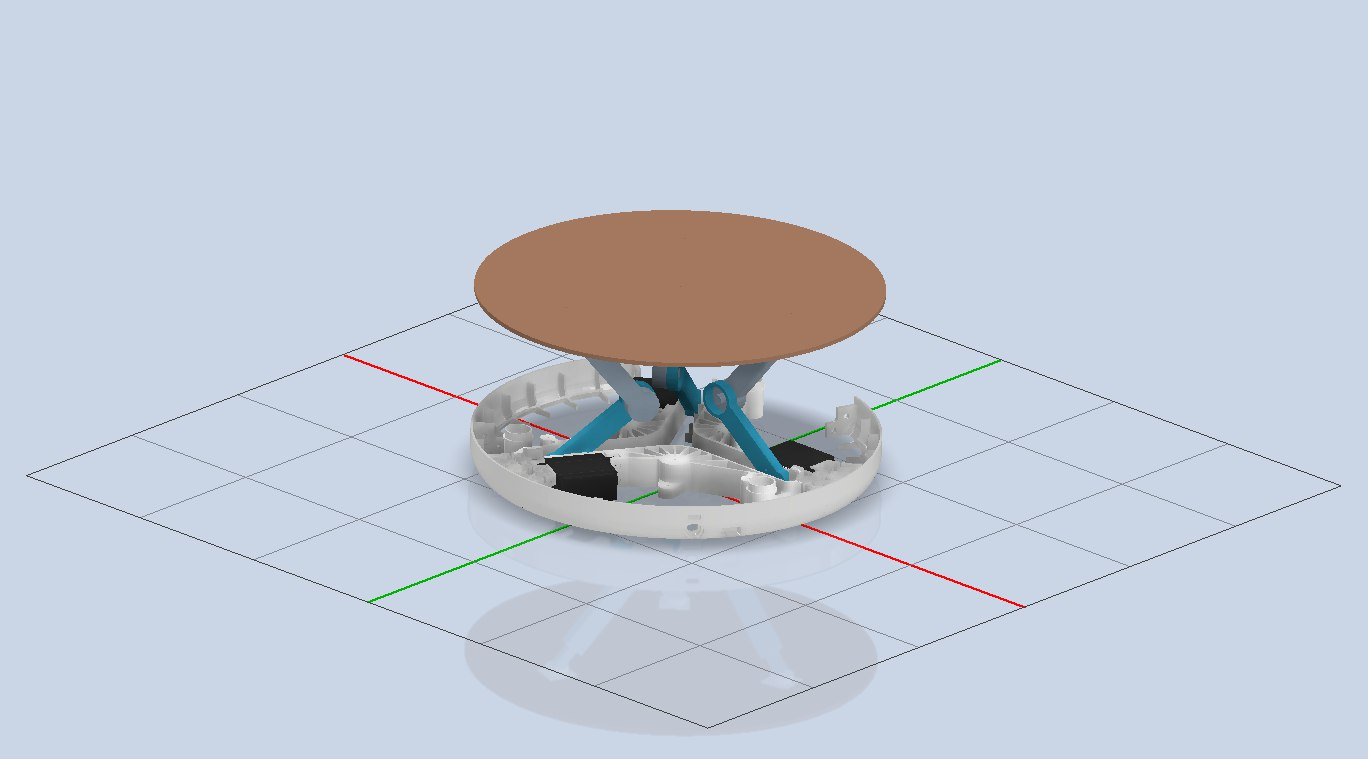
\includegraphics[width=5cm, keepaspectratio]{imports/Inventor Assambly.jpg}
        \caption{Assembly 3D made by Inventor Software with CAD pieces.}
        \label{3D Inventor assembly figure}
    \end{figure}
\end{center}

    This software allowed us to precisely manipulate the position and joint conditions between components and then export them as a block diagram to the MATLAB Simulink environment using the Simscape\cite{noauthor_simscape_nodate} library.

    \paragraph{Simulink model.}

Due to the nature of the project its export and development in the MATLAB Simulink environment was imperative, thanks to the use of the Simscape export library it was possible to transform the CAD model into a block diagram that allowed its numerical and precise manipulation to later concatenate the mechanical subsystem obtained with the ball detection system and processing of the input angles.

In the Figure \ref{Block diagram obtained by Simscape},it is evident that the input to the joints [0 to 2] corresponds to the angles to be taken by the servomotor shaft, in this case they are constant but it is there where the connection of this subsystem to the outputs of the ball detection subsystem will be made, The rotational joints [3 ... 5] correspond to the connection between the base arm and the arm connected to the plate, likewise there are 3 spherical joints that join the plate to the second arm allowing the movement of 3 degrees of freedom, shown in the Figure \ref{3D animation generated by Simulink run} an image of the execution of this subsystem.
\begin{center}
    \begin{figure}[ht!]
        \centering
        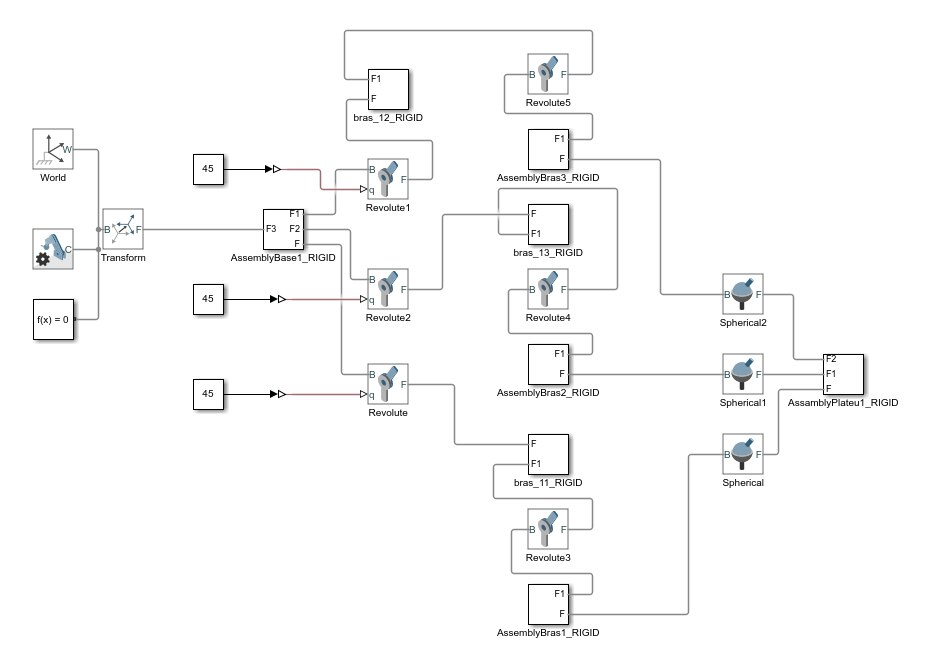
\includegraphics[width=8cm, keepaspectratio]{imports/diagrammeblocs.jpg}
        \caption{Block diagram obtained by Simscape}
        \label{Block diagram obtained by Simscape}
    \end{figure}
\end{center}

\begin{center}
    \begin{figure}[ht!]
        \centering
        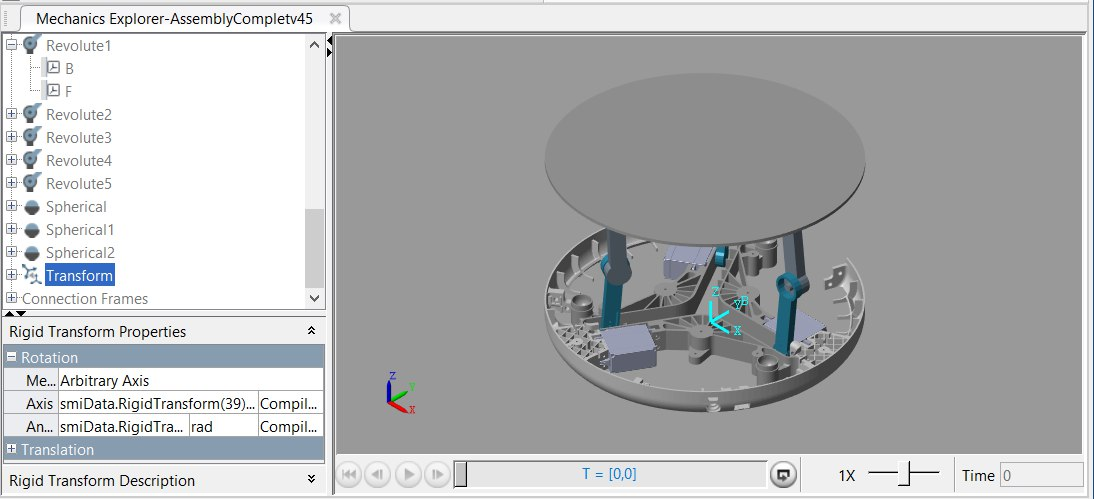
\includegraphics[width=8cm, keepaspectratio]{imports/ballandplateMatlab.jpg}
        \caption{3D animation generated by Simulink run}
        \label{3D animation generated by Simulink run}
    \end{figure}
\end{center}
  

    

\subsection{Controller}\label{Controller Materials}
\paragraph{PID Controller.}
 The PID controller is known for its simplicity and effectiveness in regulating system behavior by continuously adjusting the control input based on error, integral, and derivative terms.The control of dynamic systems plays a crucial role in numerous scientific and industrial processes. Among various control algorithms, the PID controller has gained significant popularity due to its versatility and easy of implementation. 
\\ \\
 The PID controller comprises three main components: the proportional (P) term, the integral (I) term, and the derivative (D) term. The proportional (P) term in a PID controller contributes to the control action based on the current error between the desired setpoint and the actual system output. It directly multiplies the error by a gain factor, which determines the proportionality between the error and the control output.The integral (I) term addresses steady-state errors by considering the cumulative sum of past errors.The I term acts as a corrective measure to eliminate residual errors that may persist even when the proportional term is applied. The derivative (D) term anticipates the future behavior of the system by measuring the rate of change of the error. It calculates the derivative of the error and multiplies it by a gain factor, the derivative gain.
\\

 \begin{center}
    \begin{figure}[ht!]
        \centering
        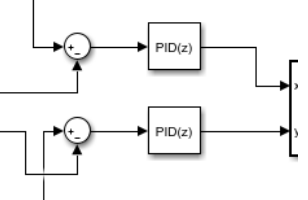
\includegraphics[width=8cm, keepaspectratio]{imports/controller-simulink.png}
        \caption{Discrete PID utilized in simulink}
        \label{Discrete PID utilized in simulink}
    \end{figure}
\end{center}

\paragraph{Controller implementation.}
The PID controller for the ball and plate system was implemented using MATLAB Simulink\cite{noauthor_simulink_nodate} and is presented in Figure \ref{Discrete PID utilized in simulink}. The control algorithm was designed to regulate the position of the ball by adjusting the plate's tilt angles. The input of the PID controller is the difference between the position of the ball and the position of the center of the plate, both in pixels, normalized, and its output is used to define the angles $\alpha$  and $\beta$  of the plate. We use a PID in discrete time\cite{noauthor_continuous-time_nodate} since the frequency of the camera and consequently of our system is 30 Hz. The Simulink block used is shown in Figure \ref{Discrete PID utilized in simulink},. And finally, PID gains were estimated with simulink's sisotool\cite{noauthor_design_nodate} tool. 
